\chapter{Arquitectura del Sistema}
\label{chap:arquitectura}

\lettrine{E}{n} este capítulo se describe la arquitectura general del sistema.
Aunque cada técnica utiliza componentes específicos para su funcionamiento,
todas se implementan sobre una misma infraestructura.

Esta decisión permite reutilizar los mecanismos de interacción con el entorno y mantener
condiciones experimentales idénticas entre las tres aproximaciones comparadas.
Las particularidades de cada una se describen en sus respectivos
Capítulos~\ref{chap:iter1}, \ref{chap:iter2} y~\ref{chap:iter3}.

\section{Arquitectura General}
El sistema se organiza en tres capas que se comunican entre sí, como se resume en
la Figura~\ref{fig:arquitectura} (página~\pageref{fig:arquitectura}):
(i) \textbf{Capa de simulación}, un servidor real de \textit{Minecraft};
(ii) \textbf{Capa de agentes}, control del agente y obtención de los estados del mundo;
y (iii) \textbf{Capa de decisión}, comunicación con los modelos de aprendizaje.

\begin{figure}[htbp]
  \centering
  \resizebox{\textwidth}{!}{%
  \begin{tikzpicture}[
    font=\footnotesize, >=Latex,
    box/.style={draw, rounded corners, align=center, minimum width=27mm, minimum height=12mm},
    lbl/.style={font=\scriptsize, align=center, inner sep=2pt},
    legbox/.style={draw, minimum width=6mm, minimum height=3mm, inner sep=0pt}
  ]
    \node[box, fill=udcpink!8]   (serv)  {SERVIDOR DE\\INFERENCIA\\{\scriptsize(\textit{Python} \textbar{} Gym Env)}};
    \node[box, fill=udcgray!8]   (ag)    [right=30mm of serv] {AGENTE\\\textit{MINEFLAYER}};
    \node[box, fill=udcgray!8]   (ag2)   [right=30mm of ag]   {SERVIDOR\\\textit{MINECRAFT}};
    \node[box, fill=ficblue!8] (data)  [above=12mm of ag]   {\textit{DATASET}};
    \node[box, fill=ficblue!8] (visor) [below=14mm of ag]   {VISOR};

    % Servidor de inferencia <-> Agente
    \draw[->] ([yshift=3mm]serv.east) -- node[lbl,above]{HTTP/INFERENCIA} ([yshift=3mm]ag.west);
    \draw[->] ([yshift=-3mm]ag.west)  -- node[lbl,below]{HTTP/ESTADO}     ([yshift=-3mm]serv.east);
    % Agente -> Dataset
    \draw[->] (ag) -- node[lbl,right]{INFO.\ STEP} (data);
    % Agente <-> Agente (agentes concurrentes)
    \draw[->] ([yshift=3mm]ag.east)   -- node[lbl,above]{ACCIONES agente}     ([yshift=3mm]ag2.west);
    \draw[->] ([yshift=-3mm]ag2.west) -- node[lbl,below]{CONOCIMIENTO agente} ([yshift=-3mm]ag.east);
    % Visor -> Agente
    \draw[->] (visor) -- node[lbl,right]{VISIÓN agente} (ag);
    % Visor -> Servidor (entrada visual)
    \draw[->] (visor.west) -| node[lbl,below,pos=0.25]{IMÁGENES} (serv.south);

    % --- LEYENDA (Abajo a la derecha) ---
    \coordinate (legend_pos) at ($(ag2.east |- visor.south) + (0,-12mm)$);
    \node[lbl, anchor=east] (ljs_text) at (legend_pos) {HTN + IL + RL};
    \node[legbox, fill=udcgray!8, left=1.5mm of ljs_text, anchor=east] (ljs) {};

    \node[lbl, left=6mm of ljs, anchor=east] (lpy_text) {IL + RL, No HTN};
    \node[legbox, fill=udcpink!8, left=1.5mm of lpy_text, anchor=east] (lpy) {};
  \end{tikzpicture}
  }
  \caption[Arquitectura general del sistema]{Arquitectura general del sistema. La capa de decisión (\textit{Python}, servidor de
  inferencia para \gls{il} y entorno \gls{gymnasium} para \gls{rl}) se comunica por \acrshort{http} con el
  agente. La \gls{htn} reside por completo en el agente, sin capa de decisión.}
  \label{fig:arquitectura}
\end{figure}

\subsection{Capa de Simulación}
Como se menciona en el Capítulo~\ref{chap:sota}, la mayoría de los trabajos
relacionados con \textit{Minecraft} emplean entornos de simulación propios, basados en versiones
modificadas del juego como \textit{MineRL}~\cite{guss2019minerl}. Sin embargo, muchas
de estas librerías están actualmente abandonadas y presentan problemas de
compilación~\cite{minerl_issue788}, por lo que se opta por un servidor real de
\textit{Minecraft} lanzado en modo \gls{headless} basado en \textit{Paper}\footnote{Una implementación de alto rendimiento del
servidor de \textit{Minecraft}.}~\cite{papermc}.

El mundo utilizado tiene la misma \gls{semilla}\footnote{Código numérico que funciona como plantilla para generar el mapa. Determina dónde
aparecen los biomas, las estructuras, los minerales y el terreno, de modo que la misma \gls{semilla} produce
siempre el mismo mundo.} en todas las iteraciones para evitar mundos donde el agente aparezca en \glspl{bioma} sin árboles
y garantizar el mismo entorno de prueba para todas las técnicas.

Si bien usar el mismo mundo podría limitar la generalización,
se introduce un mecanismo de reinicio con puntos de aparición aleatorios para aportar cierta diversidad de escenarios.

Esta diversidad de escenarios y la reproducibilidad de los episodios se basan en un
reinicio determinista. El reinicio de episodio elimina al agente del mundo y lo teletransporta
a una posición de aparición fija (la primera al entrar al mundo), de modo que cada episodio comienza
con la misma posición dentro del mismo mundo, condición necesaria para que el agente pueda explorar el entorno.
El reinicio de mundo detiene el servidor, borra el mundo y arranca uno nuevo; se puede emplear la misma \gls{semilla}
(para repetir el mismo escenario) o una aleatoria (para generar mundos aleatorios y evaluar la
generalización en distintos entornos).

El agente se conecta al servidor como un jugador mediante
\textit{Mineflayer}~\cite{mineflayer}, una \acrshort{api} en \textit{Node.js}~\cite{nodejs} que
actúa como interfaz entre el código del agente y el mundo de \textit{Minecraft}.

A través de ella se leen las percepciones (posición, orientación,
inventario y bloques cercanos) y se envían las acciones (movimiento,
rotación de cámara, minado e interacción con bloques). La percepción visual
se obtiene de \textit{prismarine-viewer}, un plugin de \textit{Mineflayer} que
renderiza la vista en primera persona del agente en un puerto local (véase el Apéndice~\ref{apx:frame});
\textit{Puppeteer}~\cite{puppeteer} captura esas imágenes y las envía a los
modelos o las guarda en disco para el \textit{dataset} de entrenamiento.

\subsection{Capa de agentes}
Toda la lógica de control gira en torno a una clase base,
\textit{BaseAgent} (Figura~\ref{fig:base-agent}, página~\pageref{fig:base-agent}),
que contiene elementos comunes de los agentes: conexión, punto de aparición en el mundo,
inicialización del visor en primera persona, gestión de errores y desconexión limpia liberando puertos y
recursos. De ella heredan las tres implementaciones de las técnicas:

\begin{figure}[htbp]
  \centering
  \resizebox{\textwidth}{!}{%
  \begin{tikzpicture}[
    font=\footnotesize, >=Latex,
    cls/.style={draw, rounded corners=2pt, align=center, minimum width=26mm, minimum height=10mm},
  ]
    \node[cls, fill=udcpink!8] (base) {\textit{BaseAgent}\\{\scriptsize conexión $\cdot$ spawn $\cdot$ percepción}};
    \node[cls, fill=udcgray!8] (il)  [below=16mm of base] {\textit{ILAgent}};
    \node[cls, fill=udcgray!8] (htn) [left=10mm of il]    {\textit{HTNAgent}};
    \node[cls, fill=udcgray!8] (rl)  [right=10mm of il]   {\textit{RLAgent}};

    % Tronco desde BaseAgent, barra horizontal y flechas hacia cada hijo
    \coordinate (bus) at ($(base.south)+(0,-8mm)$);
    \draw[semithick] (base.south) -- (bus);
    \draw[semithick] (htn.north |- bus) -- (rl.north |- bus);
    \draw[->, semithick] (htn.north |- bus) -- (htn.north);
    \draw[->, semithick] (il.north  |- bus) -- (il.north);
    \draw[->, semithick] (rl.north  |- bus) -- (rl.north);
  \end{tikzpicture}
  }
  \caption[Jerarquía de clases de la capa de agentes]{Jerarquía de clases de la
  capa de agentes. La clase base \textit{BaseAgent} concentra la conexión, el
  punto de aparición y la percepción comunes; de ella heredan \textit{HTNAgent},
  \textit{ILAgent} y \textit{RLAgent}, cada una con su propia lógica de decisión.}
  \label{fig:base-agent}
\end{figure}

\begin{itemize}
  \item \textit{HTNAgent}: ejecuta la \gls{htn}
        directamente, sin intervención externa. Su lógica reside por
        completo en las capas de \textit{Agente} y \textit{Simulación}.
  \item \textit{ILAgent}: en cada paso captura una imagen del visor, la envía al
        servidor de inferencia, recibe la acción predicha (acción discreta
        y delta de cámara) y la ejecuta.
  \item \textit{RLAgent}: actúa como puente entre el entorno \gls{gymnasium} y el agente,
        exponiendo un servidor \acrshort{http} que recibe acciones, las ejecuta y devuelve la
        observación y los eventos.
\end{itemize}

Las tres técnicas comparten la conexión y la percepción, pero difieren en la forma en que deciden la siguiente
acción. Los cambios particulares de las implementaciones se detallan en sus respectivos
Capítulos~\ref{chap:iter1}, \ref{chap:iter2} y~\ref{chap:iter3}.

\subsection{Capa de decisión}
La comunicación entre la capa de decisión (\textit{Python}) y la de agentes (\textit{Node.js}) se
realiza por \acrshort{http} con formatos \acrshort{json}. Se emplean dos canales
según la técnica:

\begin{itemize}
    \item \textbf{Imitación}: el \textit{ILAgent} actúa como cliente de un servidor
        de inferencia \textit{Python} con un \gls{endpoint}
        \textit{/predict}, al que envía la imagen del visor y el vector de estado,
        y del que recibe la acción predicha por el modelo.
    \item \textbf{Refuerzo}: el \textit{RLAgent} levanta un servidor \acrshort{http}
        con tres \textit{endpoints}: \textit{/step}, que recibe una acción,
        la ejecuta y devuelve la nueva observación junto con los eventos
        (bloques rotos, ataque a un árbol, muerte del agente\ldots); \textit{/reset},
        que reinicia el episodio; y \textit{/world\_reset}, que regenera el mundo.
\end{itemize}

\section{Entorno de simulación: Minecraft}
Como ya se describió en el Capítulo~\ref{chap:introduccion}, \textit{Minecraft} es un videojuego
\textit{3D} de mundo abierto en primera persona, basado en bloques y de generación procedimental. La
Figura~\ref{fig:minecraft_view} (página~\pageref{fig:minecraft_view}) muestra la vista en primera persona de
un jugador humano, y la Figura~\ref{fig:3d_axis} (página~\pageref{fig:3d_axis}) muestra el sistema de coordenadas que define su
orientación y posición en el mundo.

\begin{figure}[htbp]
    \centering
    \begin{subfigure}[b]{0.48\textwidth}
        \centering
        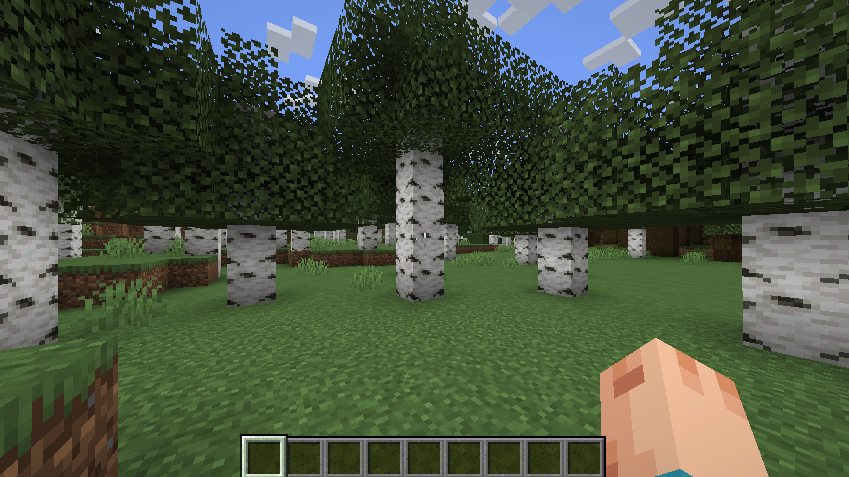
\includegraphics[width=\textwidth]{imaxes/05_arquitectura/minecraft.png}
        \caption{Vista en primera persona de un \gls{bioma} bosque.}
        \label{fig:minecraft_view}
    \end{subfigure}
    \hfill
    \begin{subfigure}[b]{0.48\textwidth}
        \centering
        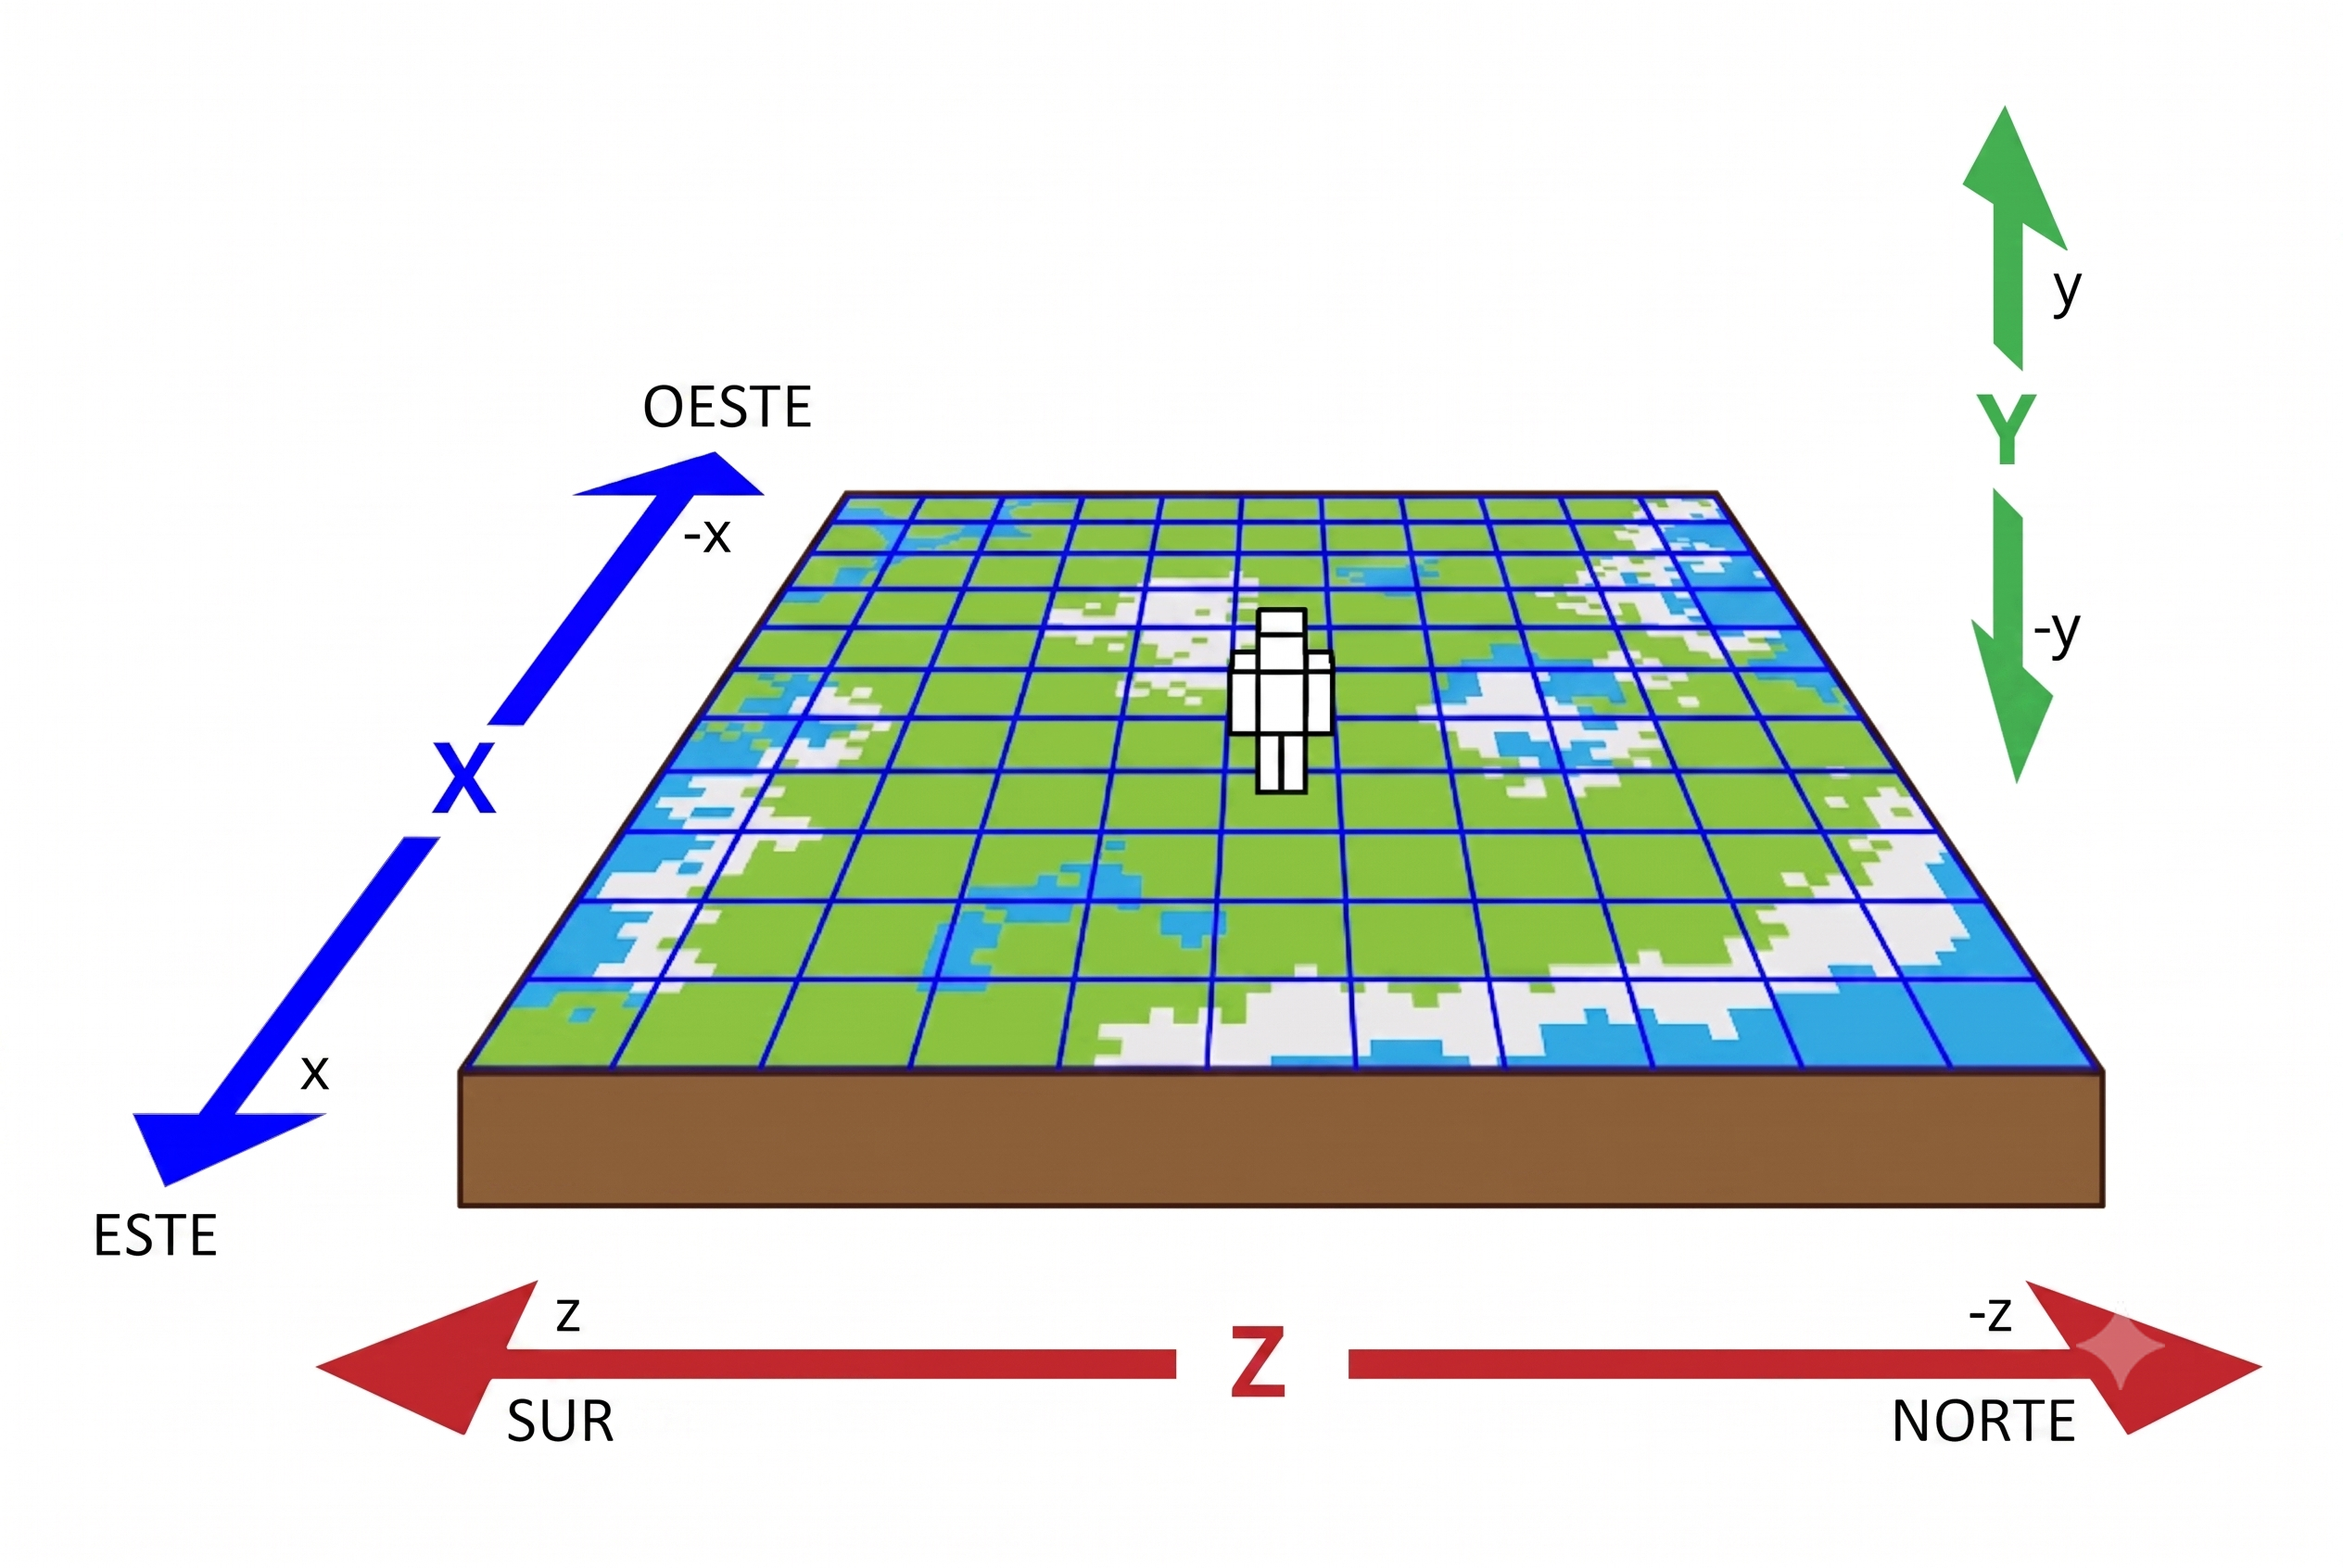
\includegraphics[width=\textwidth]{imaxes/05_arquitectura/3d_axis.png}
        \caption{Sistema de coordenadas 3D del entorno.}
        \label{fig:3d_axis}
    \end{subfigure}
    \caption[Entorno espacial de \textit{Minecraft}]{Entorno espacial de \textit{Minecraft}: vista en primera persona con el
    \gls{hud} activado (izquierda) y representación del sistema de coordenadas (derecha).}
    \label{fig:minecraft_entorno}
\end{figure}

A diferencia de juegos \textit{2D} como \textit{Atari Breakout}~\cite{DBLP:journals/nature/MnihKSRVBGRFOPB15}, el entorno
\textit{3D} introduce una nueva dimensión de complejidad, dificultando así las tareas de navegación,
orientación y percepción visual.

\section{Formulación de la tarea}
La tarea común a todas las técnicas es el \gls{woodcutting}. El agente
debe localizar un árbol, navegar hacia él, talarlo y recoger la madera.

Esta acción es la que realizaría cualquier jugador humano al comenzar a jugar a \textit{Minecraft}, y es el
primer paso de la jerarquía de progresión del juego. Aunque parezca una tarea sencilla desde la perspectiva humana,
presenta una gran dificultad para los agentes autónomos: percepción visual, navegación,
orientación de la cámara, reconocimiento de objetos, recompensa compleja\ldots En las siguientes secciones
se detallan los elementos comunes de la formulación de la tarea, adaptados posteriormente a cada técnica.

\subsection{Espacio de observaciones}
El vector de estado se compone de ocho elementos. Las variables continuas (\textit{yaw}, \textit{pitch},
\textit{dx}, \textit{dz}, \textit{tree\_distance} y \textit{log\_count}) se escalan al rango $[-1,1]$ mediante
límites fijos conocidos del entorno, propios de cada variable: los ángulos \textit{yaw} y \textit{pitch} a
$[-\pi,\pi]$ y $[-\pi/2,\pi/2]$ respectivamente; los desplazamientos del movimiento \textit{dx} y \textit{dz} se recortan a $[-1,1]$
ya que el agente avanza como máximo un bloque por paso; \textit{tree\_distance} a $[0,40]$ bloques (en un
\gls{bioma} de bosque siempre hay un árbol cerca); y \textit{log\_count} a $[0,64]$ (un \gls{stack}
de inventario). Las variables binarias (\textit{tree\_visible} e \textit{is\_looking\_at\_log}) se transforman
a $\{-1,1\}$ para mantener una escala homogénea en las entradas de la red~\cite{DBLP:series/lncs/LeCunBOM12}.
La Tabla~\ref{tab:obs-space} (página~\pageref{tab:obs-space}) resume los elementos del vector de estado.

\begin{table}[htbp]
  \centering
  \resizebox{\textwidth}{!}{%
  \small
  \rowcolors{2}{white}{udcgray!25}
  \begin{tabular}{c|c|c}
  \rowcolor{udcpink!25}
  \textbf{Componente} & \textbf{Rango} & \textbf{Descripción} \\\hline
  \textit{yaw}               & $[-\pi,\pi]$     & Orientación horizontal de la cámara (rad) \\
  \textit{pitch}             & $[-\pi/2,\pi/2]$ & Orientación vertical de la cámara (rad) \\
  \textit{dx}                & $[-1,1]$         & Desplazamiento en X respecto al paso anterior \\
  \textit{dz}                & $[-1,1]$         & Desplazamiento en Z respecto al paso anterior \\
  \textit{tree\_visible}     & $\{-1,1\}$       & Indicador de árbol visible en el cono de visión \\
  \textit{tree\_distance}    & $[0,40]$         & Distancia al árbol visible más cercano \\
  \textit{log\_count}        & $[0,64]$         & Troncos acumulados en el inventario \\
  \textit{is\_looking\_at\_log} & $\{-1,1\}$    & Indicador de cursor apuntando a un tronco \\
  \end{tabular}%
  }
  \caption[Elementos del vector de estado]{Elementos del vector de estado.}
  \label{tab:obs-space}
\end{table}

La posición absoluta $(x, y, z)$ se excluye del vector de estado de los agentes
para favorecer la generalización. Con coordenadas absolutas, el agente podría tender a memorizar posiciones
concretas del mundo en lugar de aprender a talar. En su lugar se conservan los
desplazamientos entre pasos $(dx, dz)$, que aportan información útil.
Del mismo modo, solo se conserva el desplazamiento horizontal $(dx, dz)$ y se omite el vertical $(dy)$.
En el \gls{bioma} utilizado el movimiento vertical es prácticamente nulo, por lo que aportaría un
componente casi constante y sin información, al ser la mayoría de los valores 0. Además, la entrada visual 
codifica de manera implícita la altura del agente respecto a su entorno, 
aportando un contexto espacial mucho más rico y útil que la inclusión de una coordenada vertical en el vector de estado.
Cuando se habilita la entrada visual, además del vector de estado, la red recibe una imagen \acrshort{rgb} de
\num{128} $\times$ \num{128} píxeles capturada del visor en primera persona.
En ambos casos se admite el \gls{frame-stacking}, repetir las últimas
$k$ observaciones, para dar información temporal a la red.

\subsection{Espacio de acciones}
El espacio de acciones utilizado consta de siete acciones recogidas en la
Tabla~\ref{tab:action-space} (página~\pageref{tab:action-space}).
La cámara se discretiza en giros fijos: \qty{0.15}{rad} ($\approx$ \ang{8.6})
en horizontal y \qty{0.10}{rad} ($\approx$ \ang{5.7}) en vertical. Se utiliza esta
granularidad para conseguir un cambio de estado real, sin que el agente gire la cámara manteniéndose en el mismo estado.

\begin{table}[htbp]
  \centering
  \resizebox{\textwidth}{!}{%
  \small
  \rowcolors{2}{white}{udcgray!25}
  \begin{tabular}{c|c}
  \rowcolor{udcpink!25}
  \textbf{Acción} & \textbf{Efecto} \\\hline
  \textit{attack}                & Minar el bloque apuntado por el cursor \\
  \textit{move\_forward\_sprint} & Avanzar corriendo \\
  \textit{move\_forward\_jump}   & Avanzar corriendo con salto \\
  \textit{camera\_right}         & Girar la cámara a la derecha \\
  \textit{camera\_left}          & Girar la cámara a la izquierda \\
  \textit{camera\_up}            & Subir la cámara \\
  \textit{camera\_down}          & Bajar la cámara \\
  \end{tabular}%
  }
  \caption[Espacio de acciones discreto]{Espacio de acciones discreto.}
  \label{tab:action-space}
\end{table}

\subsection{Condiciones de terminación y éxito}
Un episodio puede finalizar de tres formas. La primera es el \textbf{éxito}: recoger al menos el
número de troncos objetivo $k$ y, además, haber roto al menos
un tronco durante el episodio. Esta segunda condición previene un comportamiento espurio
donde el agente recoge troncos de episodios anteriores sin talar nuevos árboles.

La segunda forma es la \textbf{terminación anticipada}, que se dispara si el agente muere o si la
recompensa acumulada cae por debajo de un umbral, cortando episodios sin progreso. Al ser un final
real de la tarea, se deja el valor del estado siguiente a cero.

La última forma es el \textbf{truncamiento}, al alcanzar el número máximo de
pasos por episodio. A diferencia de la terminación, el valor del estado siguiente no es cero,
lo que indica al agente que el episodio aún podría continuar.

\subsection{Percepción del entorno}
El componente principal de la percepción es la detección de árboles. Si bien el agente
podría obtener un conocimiento omnisciente del mundo a través de la \acrshort{api} de \textit{Mineflayer} (conociendo la
posición exacta de cualquier bloque, enterrado o tras un muro), se limita
la información que recibe para simular lo máximo posible la percepción de un jugador humano.

Para ello, la búsqueda de troncos se restringe al
\gls{fov} del agente, evitando información sobre objetos
que no podría ver. Además, para percibir un objeto el agente debe tener una línea de
visión directa hacia él.

La detección comienza con la función \textit{findBlocks} de \textit{Mineflayer}, que devuelve
las posiciones de los bloques de un tipo dado dentro de un radio fijo (por defecto, \num{32} bloques)
alrededor del agente. Los bloques devueltos por la función vienen ordenados por cercanía al agente. Sobre esos candidatos se aplica un
filtro en tres etapas, devolviendo el primer bloque que las supera todas:

\begin{enumerate}
  \item \textbf{Cara expuesta}: el bloque debe tener al menos una cara al aire. Esto
        asegura que el bloque es visible y accesible directamente.
  \item \textbf{Cono de visión}: el bloque debe estar dentro del campo de visión
        del agente, cono de \ang{90} en horizontal y
        \ang{60} en vertical respecto a la orientación (\textit{yaw}, \textit{pitch})
        del agente.
  \item \textbf{Línea de visión}: se traza un \gls{raycast} (línea proyectada desde un punto fijo en una dirección concreta)
        desde los ojos del agente hasta el bloque, el cual debe alcanzarse sin chocar previamente con otro bloque sólido
        (elementos como el agua no bloquean la visión).
\end{enumerate}

De este modo, el agente solo conoce los árboles que un jugador podría realmente
ver en ese instante.

\subsection{Reproducibilidad}
La reproducibilidad del sistema se basa en el uso del mismo mundo y \gls{semilla} en todas las iteraciones y en los
reinicios deterministas a una posición de aparición fija. Así, todas las técnicas se entrenan y evalúan bajo
idénticas condiciones, variando únicamente en la posición inicial al generar el mundo, lo que garantiza que las comparaciones 
entre las familias de algoritmos del Capítulo~\ref{chap:discusion-resultados} sean justas.